\cleardoublepage

\section{方案构思}

\subsection{设计创新点以及设计源点}

\subsubsection{设计源点}

本方案的设计源点在于原生三维纹理生成模型与图像扩散模型之间存在的先验鸿沟。
原生三维生成模型直接在三维空间中对几何与纹理进行联合建模，
具备天然的视角一致性与几何对齐优势，能够在单次前向推理中输出完整的三维资产。
然而，受制于高质量三维数据的获取成本，
现有三维数据集在规模与多样性上与二维图像数据集相比仍存在数量级的差距，
导致此类模型对物体外观细节的感知与推断能力相对有限。
这一局限在处理遮挡区域、背面纹理以及细粒度材质细节时尤为突出——
模型往往因缺乏足够的外观先验而倾向于生成模糊、失真或语义错误的纹理。
相比之下，以Stable Diffusion为代表的图像扩散模型经过海量二维图像数据的训练，
积累了极为丰富的外观先验，对物体纹理、材质、光照及风格均具有更强的感知与推断能力，
能够合成高度真实、细节丰富的图像内容。
如何将这一丰富的二维外观先验有效迁移至三维生成过程，
是本文方案设计的核心出发点。

如图~\ref{fig:weakness}~所示，
在仅以单张正面参考图直接驱动原生三维纹理生成时（图~\ref{fig:weakness}~第二列），
由于模型对背部区域的外观先验严重不足，
模型无法从单一正面视角推断出背部的合理外观，
将原本属于外部工装衣的区域错误识别为内部背心，
导致生成结果与真实物体外观存在明显的语义偏差。
这一现象并非个例，而是当前原生三维生成模型在面对外观信息不完整的输入时的普遍缺陷，
反映了其在外观推断能力上的系统性局限。

为此，本文提出的方案（图~\ref{fig:weakness}~第三列）采用两阶段策略加以应对：
首先通过多视角扩散模型由单张参考图补全各视角的外观信息，
生成视角一致、细节丰富的多视角图像序列；
再以这些多视角图像为条件，引导经LoRA微调后的Trellis.2进行三维纹理生成。
这一设计有效将图像扩散模型中蕴含的丰富二维外观先验桥接至三维生成过程，
使模型在生成背部、侧面等遮挡区域时能够参考更为完整的外观信息，
从而显著提升生成结果的语义正确性与材质保真度。
从实验结果来看，本文方案生成的背部纹理在色彩、材质与结构细节上
均与真值（GT，图~\ref{fig:weakness}~第四列）更为吻合，
明显优于直接以单视图驱动的基线结果，
验证了多视角先验注入策略在弥补原生三维模型外观推断缺陷方面的有效性。

\begin{figure}[t]
    \centering
    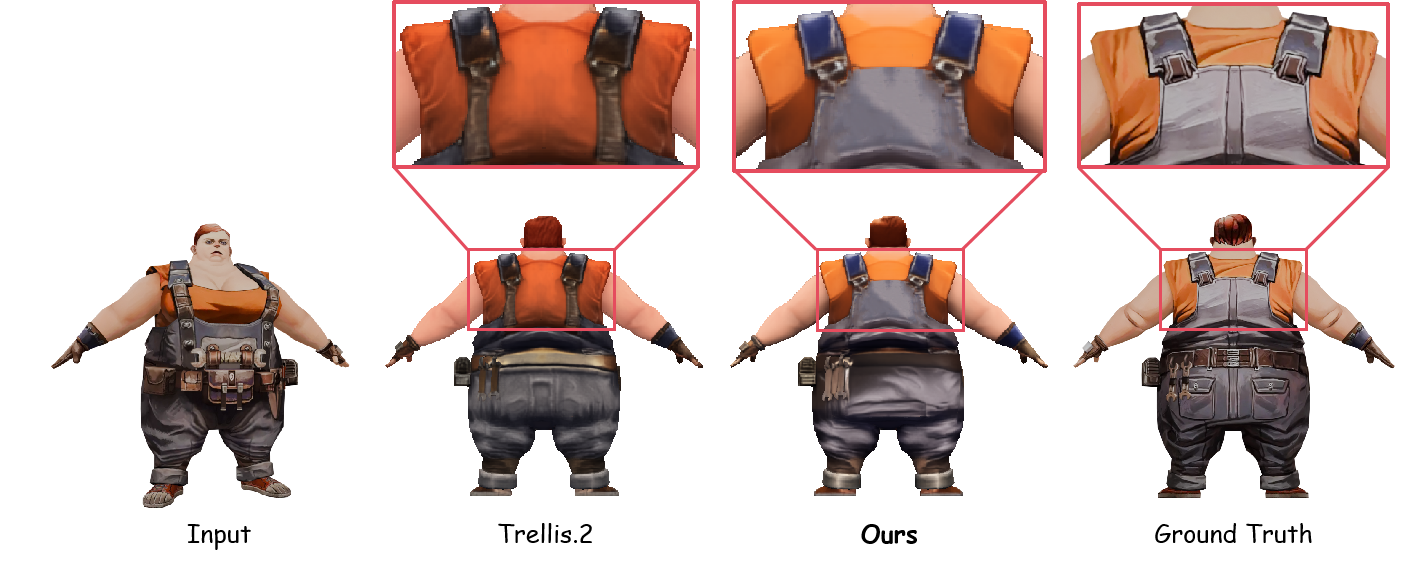
\includegraphics[width=\linewidth]{figure/final/weakness.png}
    \caption{
        单视角输入下的纹理生成对比。
        从左至右依次为：参考图（Reference）、
        直接以参考图驱动 Trellis.2 生成的结果（Trellis.2）、
        本文方案生成结果（Ours）及真值（Ground Truth）。
        放大的背部区域表明，引入多视角扩散先验后，
        本文方案在遮挡区域的纹理质量上取得了显著提升。
    }
    \label{fig:weakness}
\end{figure}

如何在不破坏原生三维生成模型固有能力的前提下，
将图像扩散模型中蕴含的丰富二维先验迁移并注入三维生成过程，
是本文的核心出发点。

\subsubsection{设计创新点}

针对上述问题，本方案提出以下创新点：

\begin{enumerate}

  \item \textbf{多视角先验引入。}
  引入 MV-Adapter 作为多视角图像合成模块，
  以单张输入图像为条件生成多视角一致图像序列，
  将图像扩散模型中蕴含的丰富外观先验转化为可供三维生成模型直接利用的多视角条件信号，
  有效弥补了原生三维模型在外观先验方面的不足。

  \item \textbf{参数高效的多视角条件注入。}
  提出对 Trellis.2 扩散网络进行低秩自适应（LoRA）\cite{hu2022lora}微调，
  针对网络中每个 Transformer Block 的自注意力与交叉注意力层引入低秩旁路，
  以少量可训练参数实现多视角条件信号的高效注入，
  在显著降低训练成本的同时，有效保留了预训练模型原有的三维生成能力。

  \item \textbf{单视图到三维的完整生成框架。}
  将多视角图像合成与多视角条件三维生成两个阶段有机串联，
  构建了一套从单张图像出发、端到端生成高质量三维资产的完整框架，
  在几何完整性、材质保真度和跨视角一致性方面均有明显提升。

\end{enumerate}

\subsection{用户调研}
为了分析自动三维生成技术的用户需求及使用场景，本研究采用半结构化访谈的方法，
对三维内容创作者进行了深入调研。访谈旨在了解用户群体特征、
使用频率、主要应用场景以及对自动化生成工具的需求与体验\cite{陈向明2000质的研究方法}。

\subsubsection{调研方法}

本次用户调研主要采用半结构化访谈与问卷结合的方式。访谈对象涵盖：

\begin{itemize}
  \item \textbf{专业用户}：游戏开发人员、影视特效师、三维建模师，共 3 名。
  \item \textbf{非专业用户}：三维内容创作爱好者、学生及自媒体创作者，共 10 名。
\end{itemize}

访谈内容包括：用户日常三维内容制作流程、对自动生成工具的使用频率、
使用中遇到的问题、对材质自动生成和迁移功能的需求，以及对未来工具改进的期望等
（详细调查提纲见附录~\ref{app:survey}）。
每次访谈时长约 30-45 分钟，记录访谈音频并整理访谈笔记。通过对问卷与访谈笔记的定性分析，总结出用户特征与使用特点。

\subsubsection{主要调研发现}

根据访谈结果，可归纳如下特点：

\begin{enumerate}
  \item \textbf{用户群体特征鲜明}：  
  大多数用户表示在日常工作或学习中频繁使用三维建模工具。访谈显示，非专业用户对自动化材质生成功能依赖度更高，专业用户则关注生成效果的可控性与多视角一致性。

  \item \textbf{使用场景广泛}：  
  用户将自动三维生成技术应用于多个场景，包括游戏关卡设计、虚拟场景搭建、影视特效制作、在线内容创作及教育培训。访谈中大多数用户表示在实际工作中希望能快速生成高质量材质，以节省人工绘制纹理的时间。

  \item \textbf{核心需求集中}：  
  通过访谈整理发现，用户对自动三维生成工具的核心需求集中于
  \begin{itemize}
    \item 快速生成符合模型结构的高质量材质贴图；
    \item 多样化的输入形式，如单视图、多视图、文本等；
    \item 提供可视化预览工具以快速评估生成结果；
    \item 简单易用的 Web 平台，降低安装和学习成本。
  \end{itemize}
\end{enumerate}

\subsubsection{用户旅程图分析}

基于访谈结果，本研究构建了用户在使用自动三维生成工具过程中的旅程图（图\ref{fig:user_journey}）。
\begin{figure}[htbp]
    \centering
    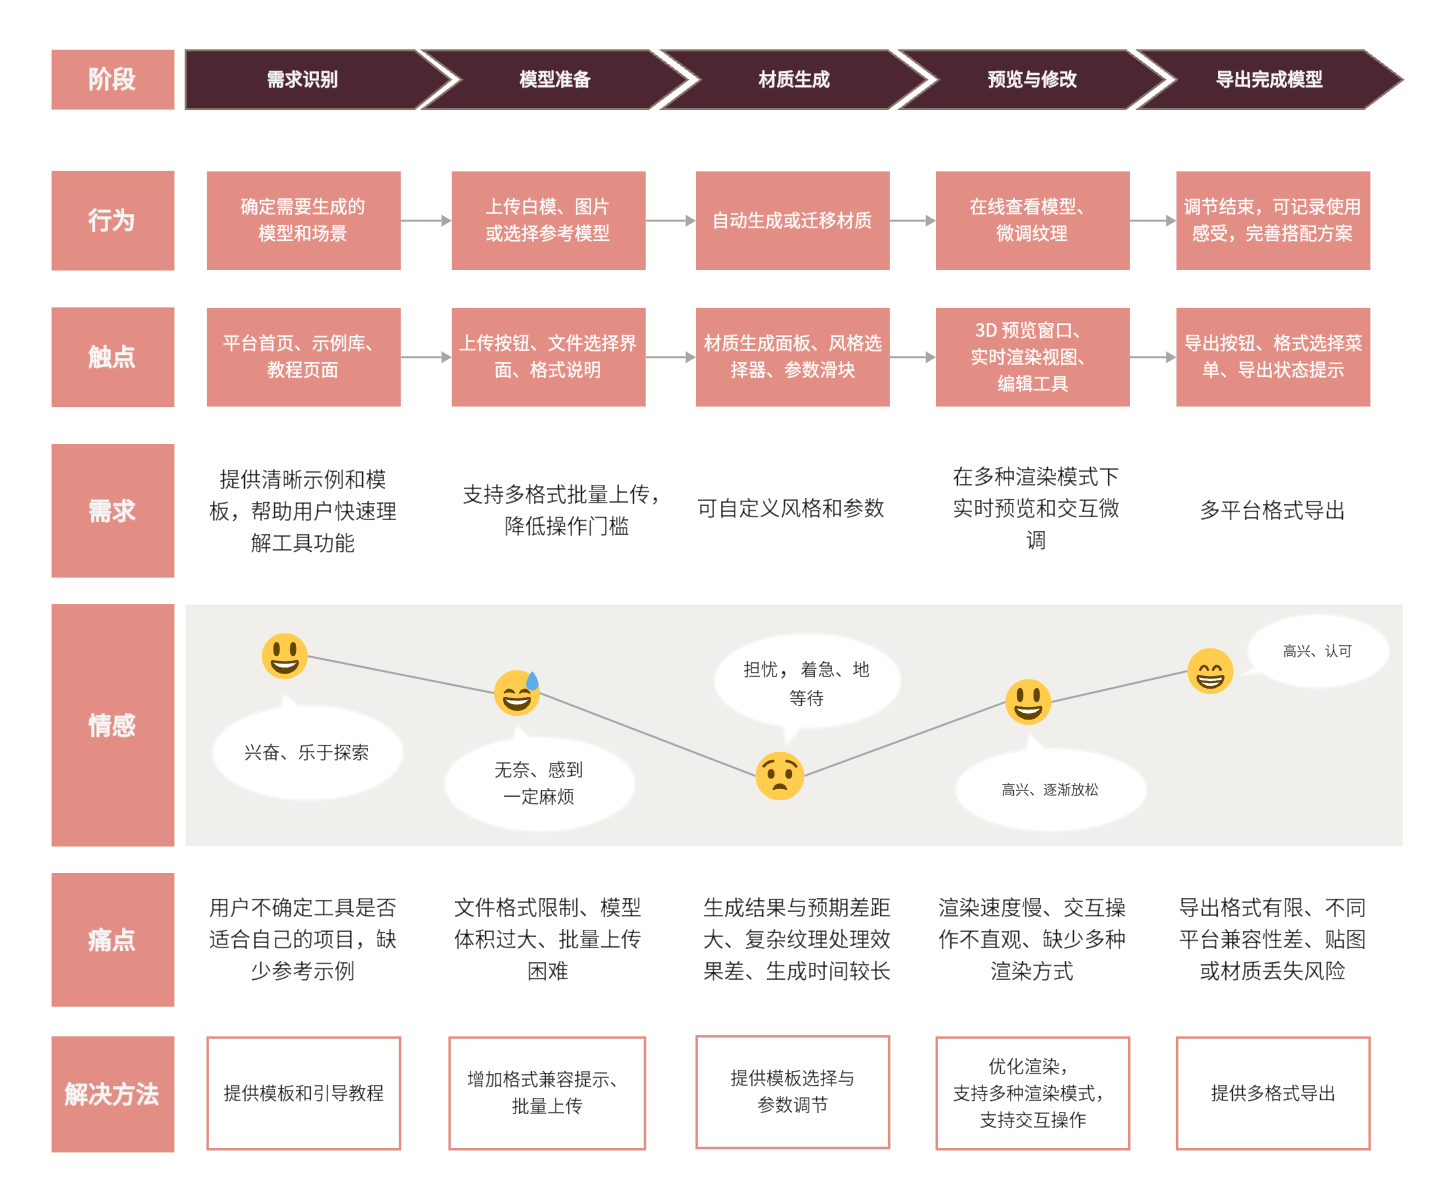
\includegraphics[width=0.8\textwidth]{figure/proposal/journey.png}
    \caption{面向 Web 三维生成系统的用户旅程图}
    \label{fig:user_journey}
\end{figure}
用户旅程分为五个阶段：需求识别、模型准备、材质生成、预览与修改及导出与应用。  

旅程图清晰展示了用户在各阶段的操作、体验情绪、痛点以及对工具的需求。
在材质生成阶段，用户普遍对生成效果不够精细和风格不统一感到沮丧。
深入分析用户反馈可以发现，这一痛点的根源在于现有工具普遍仅支持单视图输入，
导致模型无法感知完整的外观信息，生成结果缺乏全局一致性。
对此，用户明确表达了两类核心诉求：
其一，希望系统支持直接输入多视角参考图像，以提供更丰富的外观约束，从而生成风格统一、细节精准的纹理；
其二，在多视角参考图像不可得时，期望系统能够先由单张参考图自动推断并生成多视角图像，
再以此为基础驱动纹理生成，以兼顾操作便捷性与生成质量的验证效率。

上述需求揭示了现有方法在多视角感知与利用上的显著缺口。
为此，本文提出一种多视角引导的三维纹理生成框架：
在多视角输入可用时，直接以多视角图像为条件约束生成过程；
在仅有单视图时，则先通过多视角扩散模型补全视角信息，再完成纹理生成。
这一设计不仅切实回应了用户的核心痛点，也构成了本工作的核心动机与主要贡献。

